\documentclass[a4paper,10pt]{article}
\usepackage[utf8]{inputenc}
\usepackage{enumerate}
\usepackage{amsmath}
\usepackage{graphicx}
\usepackage{listings}
\usepackage{float}
\usepackage[caption = false]{subfig}
\usepackage[parfill]{parskip}
\usepackage{url}

\title{Project 1}
\author{Candidate number: 15025\footnote{I have collaborated with another student.}}
\date{2018}

\begin{document}
\maketitle

When refering to equations from the task sheet I will add a star (e.g. "equation (1*)"). The plots are forced into the correct place, for the benefit of the reader.

\section{Analytical tasks}
Following are the answers to the question where the number of the task answered is given by the number of the subsection.

\subsection{Energy density of the scalar field}
Inserting the definition of the Hubble parameter in equation (8*) we get 

\begin{align}
\frac{d\rho_{\phi}}{dt} = -3\frac{\dot{a}}{a}\rho_{\phi}(1+w_{\phi}).
\end{align}

By definition $\dot{a} = da/dt$, inserting this and multiplying the equation by $dt$ yields

\begin{align}\label{eq:d_rho}
d\rho_{\phi} = -3\rho_{\phi}(1+w_{\phi})\frac{da}{a}.
\end{align}

Consider multiplying $da/a$ by $dz/dz$, sorting and using the definition of the reshift $a = a_0/1+z$

\begin{equation}
%\setlength{\jot}{10pt}
\begin{split}
\frac{da}{dz}\frac{dz}{a} &= -\frac{a_0}{(1+z)^2}\frac{dz}{a}  \\
&= -\frac{a_0}{(1+z)^2} \frac{(1+z) dz}{a_0} \\
&= -\frac{1}{1+z} dz
\end{split}
\end{equation}

Inserting the above equation into \eqref{eq:d_rho} and multiplying by $1/ \rho_{\phi}$, yields

\begin{align}
\frac{d\rho_{\phi}}{\rho_{\phi}} = 3\frac{(1+w_{\phi})}{1+z} dz.
\end{align}

Integrating $\rho_{\phi}$ from $\rho_{\phi0}$ to a general $\rho_{\phi}$ and $z$ from $0$ to a general $z$ we get

\begin{align}
\int_{\rho_{\phi 0}}^{\rho_{\phi}} \frac{d\tilde{\rho}_{\phi}}{\tilde{\rho}_{\phi}}  = 3 \int_0^z\frac{(1+w_{\phi})}{1+\tilde{z}} d\tilde{z}.
\end{align}

Solving the left hand integral yields $\ln(\rho_{\phi}/\rho_{\phi 0})$. Exponentiating the equation and multiplying by $\rho_{\phi 0}$

\begin{align}
\rho_{\phi} = \rho_{\phi 0} \exp\bigg( \int_0^z\frac{3(1+w_{\phi})}{1+\tilde{z}} d\tilde{z}\bigg)
\end{align}


\subsection{Time derivative of hubble parameter}
Deriving the Hubble parameter squared we have to use the chain rule since the Hubble parameter is a function of t, so that 

\begin{align*}
\frac{dH^2}{dt} = 2H\frac{dH}{dt} = \frac{d}{dt} \bigg(\frac{8\pi G}{3} \sum_i \rho_i\bigg) = \frac{8\pi G}{3} \sum_i \frac{d \rho_i}{dt}
\end{align*}

where G is the gravitational constant and the sum goes over radiation r, mass m and the scalar field $\phi$. Applying the continuity equation $d\rho_i/dt = -3H(\rho_i + p_i) = -3H\rho_i(1+w_i)$, we get

\begin{align}\label{eq:2HdH/dt}
2H\frac{dH}{dt} = \frac{8\pi G}{3} \sum_i -3H(\rho_i + p_i).
\end{align}

The sum we find to be

\begin{equation*}
\begin{split}
\sum_i (\rho_i + p_i) &= (\rho_m + p_m) + (\rho_r + p_r) + (\rho_{\phi} + p_{\phi}) \\
&= \rho_m(1 + w_m) + \rho_r(1+w_r) + (\rho_{\phi} + p_{\phi})
\end{split}
\end{equation*}

Adding the energy density and the pressure of the scalar field we get $\rho_{\phi} + p_{\phi} = (d\phi/dt)^2$. Multiplying the equation \eqref{eq:2HdH/dt} by $1/2H$, and inserting the sum above

\begin{align}
\frac{dH}{dt} = -\frac{\kappa^2}{2}\bigg[\rho_m(1+w_m) + \rho_r(1+w_r) + \bigg(\frac{d\phi}{dt}\bigg)^2\bigg].
\end{align}


\subsection{Density parameters}
We have that the density parameter is given by $\Omega_i = \rho_i/\rho_c$, where $\rho_c$ is the critical density. Following is the derivation for the density parameter of 1) the scalar field in terms of $x_1$ and $x_2$ 2) the radiation in terms of $x_3$ 3) the matter in terms of $x_1$, $x_2$ and $x_3$:

\begin{align}
\begin{split}
\Omega_{\phi} &= \frac{\rho_{\phi}}{\rho_c} = \frac{ \frac{1}{2}\dot{\phi^2} + V}{3H^2/8\pi G} = \frac{ \frac{1}{2}\dot{\phi^2} + V}{3H^2}\kappa^2 \\
&= \bigg(\frac{\dot{\phi}^2}{6H^2} + \frac{V}{3H^2}\bigg)\kappa^2 = x_1^2 + x_2^2.
\end{split}
\end{align}

Further we have 

\begin{align}
\begin{split}
\Omega_r = \frac{\rho_r}{\rho_c} = \frac{\rho_r \kappa^2}{3H^2} = x_3^2.
\end{split}
\end{align}

Since the sum of the density parameters must be 1, we have that the density parameter of the mass is 1 minus the density parameter of the other components

\begin{align}
\begin{split}
\Omega_m = 1 - \Omega_{\phi} - \Omega_r = 1 - x_1^2 - x_2^2 - x_3^2
\end{split}
\end{align}


\subsection{$\dot{H}/H^2$ in terms of x}
Multiplying equation (12*) by the inverse of the critical density $1/\rho_c$

\begin{align}
\frac{1}{\rho_c}\frac{dH}{dt} = -\frac{\kappa^2}{2}\bigg[\frac{\rho_m}{\rho_c}(1+w_m) + \frac{\rho_r}{\rho_c}(1+w_r) + \frac{\dot{\phi}^2}{\rho_c}\bigg]
\end{align}

We know that $\Omega_i = \rho_i/\rho_c$ and we have that $w_m = 0$ and $w_r = 1/3$, inserting

\begin{align}
\frac{8\pi G}{3H^2}\frac{dH}{dt} = -\frac{8\pi G}{2}\bigg[\Omega_m + \frac{4}{3}\Omega_r + \frac{\kappa \dot{\phi}^2}{3H^2}\bigg].
\end{align}

Multiplying the last equation by $3/8\pi G$ and for the last term in the bracket we simply use that $1/3 = 2/6$

\begin{equation*}
\begin{split}
\frac{\dot{H}}{H^2} &= -\frac{3}{2}\bigg[\Omega_m + \frac{4}{3}\Omega_r + 2\frac{\kappa \dot{\phi}^2}{6H^2}\bigg] \\
&= -\frac{3}{2}\bigg[1 - x_1^2 - x_2^2 - x_3^2 + \frac{4}{3}x_3^2 + 2x_1^2\bigg] \\
&= -\frac{1}{2}\bigg[3 + 3x_1^2 - 3x_2^2 + x_3^2\bigg]
\end{split}
\end{equation*}


\subsection{Derivatives of x}
Derivating $x_1$ with respect to t yeilds

\begin{align*}
\frac{dx_1}{dt} = \frac{d}{dt}\bigg(\frac{\kappa \dot{\phi}}{\sqrt{6}H}\bigg) = \frac{\kappa}{\sqrt{6}}\frac{\ddot{\phi}H - \dot{\phi}\dot{H}}{H^2}
\end{align*}

by the product rule. We know that $\ddot{\phi} + 3H\dot{\phi} + V' = 0$, solving for $\ddot{\phi}$ and inserting into the above equation:

\begin{align*}
\frac{dx_1}{dt} &= \frac{\kappa}{\sqrt{6}}\bigg(\frac{-3H\dot{\phi}-V'}{H} - \dot{\phi}\frac{\dot{H}}{H^2}\bigg)\\
&= \frac{\kappa}{\sqrt{6}}\bigg(-3\dot{\phi} - \frac{V'}{H} - \dot{\phi}\frac{\dot{H}}{H^2}\bigg) \\
&= -3\frac{\kappa \dot{\phi}}{\sqrt{6}} - \frac{\kappa V'}{\sqrt{6}H} - \frac{\kappa \dot{\phi}}{\sqrt{6}}\frac{\dot{H}}{H^2}.
\end{align*}

Further we have that $dx/dt = Hdx/dN$, and we insert $\dot{H}/H^2$:

\begin{align*}
\frac{dx_1}{dN} &= \frac{1}{H}\frac{dx_1}{dt} = -3\frac{\kappa \dot{\phi}}{\sqrt{6}H} - \frac{\kappa V'}{\sqrt{6}H^2} + \frac{\kappa \dot{\phi}}{\sqrt{6}}\frac{1}{2}(3 + 3x_1^2 - 3x_2^2 + x_3^2) \\
&=  -3\frac{\kappa \dot{\phi}}{\sqrt{6}H} - \frac{\kappa V'}{\sqrt{6}H^2} \frac{\kappa V \sqrt{6}}{\kappa V \sqrt{6}} + \frac{\kappa \dot{\phi}}{\sqrt{6}}\frac{1}{2}(3 + 3x_1^2 - 3x_2^2 + x_3^2) \\
&= -3\frac{\kappa \dot{\phi}}{\sqrt{6}H} + \frac{\sqrt{6}}{2}\frac{\kappa^2 V}{3H^2}\bigg(\frac{-V'\sqrt{6}}{\kappa V}\bigg) + \frac{1}{2}x_1(3 + 3x_1^2 - 3x_2^2 + x_3^2) \\
&= -3x_1 + \frac{\sqrt{6}}{2}x_2^2\lambda + \frac{1}{2}x_1(3 + 3x_1^2 - 3x_2^2 + x_3^2)
\end{align*}

Derivating $x_2$ with respect to t yeilds

\begin{align*}
\frac{dx_2}{dt} &= \frac{d}{dt}\bigg(\frac{\kappa\sqrt{V}}{\sqrt{3}H} = \frac{\kappa}{\sqrt{3}}\bigg(\frac{\frac{1}{2}V^{-1/2}HV'\dot{\phi} - \sqrt{V}\dot{H}}{H^2} \bigg) \\
&= \frac{\kappa}{\sqrt{3}}\bigg(\frac{V'\dot{\phi}}{2H\sqrt{V}} - \sqrt{V}\frac{\dot{H}}{H^2}\bigg).
\end{align*}

Multiplying the first part of the last equation by $\sqrt{6}\sqrt{V}\kappa/\sqrt{6}\sqrt{V}\kappa$:

\begin{align*}
\frac{dx_2}{dt} &= \frac{\kappa \dot{\phi}}{H} \frac{1}{\sqrt{3}}\frac{V'}{\sqrt{V}}\frac{1}{2}\frac{\sqrt{6}\sqrt{V}\kappa}{\sqrt{6}\sqrt{V}\kappa} - \frac{\kappa \sqrt{V}}{\sqrt{3}}\frac{\dot{H}}{H^2} \\ 
&= \frac{\kappa \dot{\phi}}{H\sqrt{6}} \frac{\kappa \sqrt{V}}{\sqrt{3}}\frac{V'}{\sqrt{V}\sqrt{V}\kappa}\frac{1}{2} - \frac{\kappa \sqrt{V}}{\sqrt{3}}\frac{\dot{H}}{H^2}
\end{align*}

by the product rule. We then have

\begin{align*}
\frac{dx_2}{dN} &= \frac{1}{H}\frac{dx_2}{dt} = x_1 \frac{\kappa \sqrt{V}}{\sqrt{3}H}(-\lambda)\frac{\sqrt{6}}{2} - \frac{\kappa \sqrt{V}}{\sqrt{3}H}\frac{\dot{H}}{H^2} \\
&= -\frac{\sqrt{6}}{2}x_1x_2\lambda + \frac{1}{2}x_2 (3 + 3x_1^2 - 3x_2^2 + x_3^2).
\end{align*}

Derivating $x_3$ with respect to t yeilds

\begin{align*}
\frac{dx_3}{dt} &= \frac{d}{dt}\bigg(\frac{\kappa \sqrt{\rho_r}}{\sqrt{3}H}\bigg) = \frac{\kappa}{\sqrt{3}}\frac{d}{dt}\bigg(\frac{\sqrt{\rho_r}}{H}\bigg) \\
&= \frac{\kappa}{\sqrt{3}}\bigg(\frac{\frac{1}{2}(\rho_r)^{-1/2}\dot{\rho_r}H}{H^2} - \frac{\sqrt{\rho_r}\dot{H}}{H^2}\bigg) \\
&= \frac{\kappa}{\sqrt{3}}\bigg(\frac{\dot{\rho_r}}{2\sqrt{\rho_r}H} - \sqrt{\rho_r}\frac{\dot{H}}{H^2}\bigg).
\end{align*}

From the lectures we know that $\dot{\rho_r} = -4H\rho_r$. So we get

\begin{align*}
\frac{dx_3}{dt} &= \frac{\kappa}{\sqrt{3}} \bigg(\frac{-4H\rho_r}{2\sqrt{\rho_r} H} - \sqrt{\rho_r}\frac{\dot{H}}{H^2}\bigg) \\
&= \frac{-2\kappa \sqrt{\rho_r}}{\sqrt{3}} - \frac{\kappa \sqrt{\rho_r}}{\sqrt{3}} \\
&= -2x_3 + x_3 \frac{1}{2}(3 + 3x_1^2 - 3x_2^2 + x_3^2).
\end{align*}


\section{Numerical part}
\subsection{Energy densities and equation of state}

The equation of state for the scalar field is given by

\begin{align}\label{eq:w_phi}
w_{\phi} = \frac{p_{\phi}}{\rho_{\phi}} = \frac{\frac{1}{2}\dot{\phi}^2 - V}{\frac{1}{2}\dot{\phi}^2 + V}.
\end{align}

We can express $\dot{\phi}$ from the expression for $x_1$ so that $\dot{\phi} = x_1\sqrt{6}H/\kappa$, further we express $H/\kappa$ from the expression for $x_2$ so that $H/\kappa = \sqrt{V}/x_2\sqrt{3}$, which yields that $\dot{\phi} = \sqrt{2V}x_1/x_2$, we insert into equation \eqref{eq:w_phi} and get

\begin{align*}
w_{\phi} &= \frac{\frac{1}{2}2V(\frac{x_1}{x_2})^2 - V}{\frac{1}{2}2V(\frac{x_1}{x_2})^2 + V} = \frac{V((\frac{x_1}{x_2})^2 - 1)}{V((\frac{x_1}{x_2})^2 + 1)} \\
&= \frac{\frac{x_1^2 - x_2^2}{x_2^2}}{\frac{x_1^2 + x_2^2}{x_2^2}} = \frac{x_1^2 - x_2^2}{x_1^2 + x_2^2}.
\end{align*}

The plots can be found in figure \ref{fig:omega_ipl} - \ref{fig:eos_exp}. From figure \ref{fig:omega_ipl} and \ref{fig:omega_exp} we can see that both models provide a universe that is radiation dominated in the beginning, and the domination of radation and matter change at approximately the same time. The model with the exponential potential has a greater matter energy density peak than that of the inverse power law, and as the redshift fades, the matter domination of the exponential model is greater. The scalar field has less of a presence in the exponential model, it begins later in time and it has a lower density in total.

\begin{figure}[H]
\centering
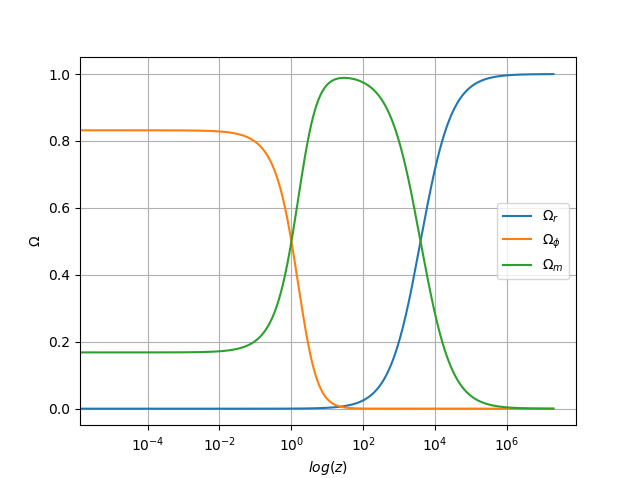
\includegraphics[width=12cm]{omega_IPL.png}
\caption{Fractional energy densities for the inverse power law potential.}
\label{fig:omega_ipl}
\end{figure}
\begin{figure}[H]
\centering
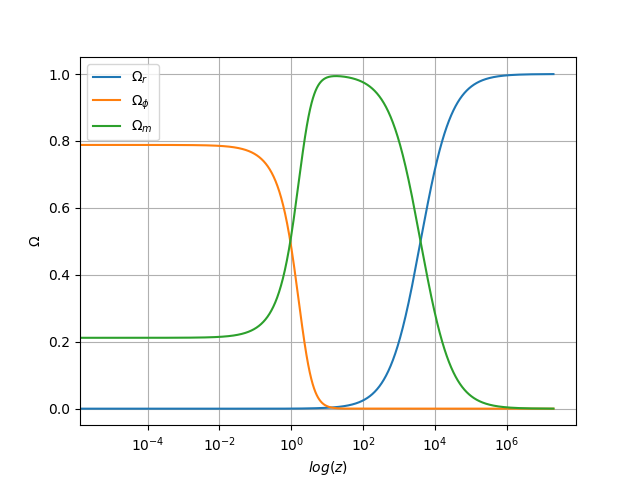
\includegraphics[width=12cm]{omega_EXP.png}
\caption{Fractional energy densities for the exponential potential.}
\label{fig:omega_exp}
\end{figure}

In figure \ref{fig:eos_exp} we see that for high valued redshift the model has an equation of state that is $-1$, which means that the potential is greater than the time derivative of the scalar field. For an equations of state $= -1$ it has the same solution as the cosmological constant, which tells us that this is a model that fits well with observations.

For the inverse power law potential we see in figure \ref{fig:eos_ipl} that for high valued redshift, the equation of state has a value of $1$, which tells us that the potential is 0, and the scalar field is free. This model also has an equation of state the same as for a cosmological constant.

\begin{figure}[H]
\centering
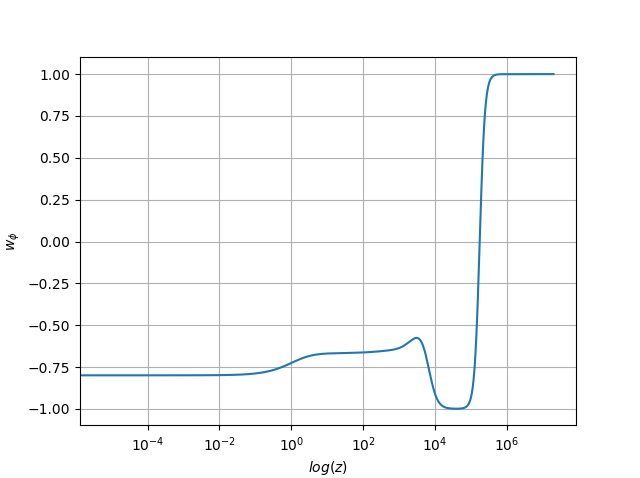
\includegraphics[width=12cm]{eos_ipl.png}
\caption{Equation of state of the scalar field for inverse power law potential.}
\label{fig:eos_ipl}
\end{figure}
\begin{figure}[H]
\centering
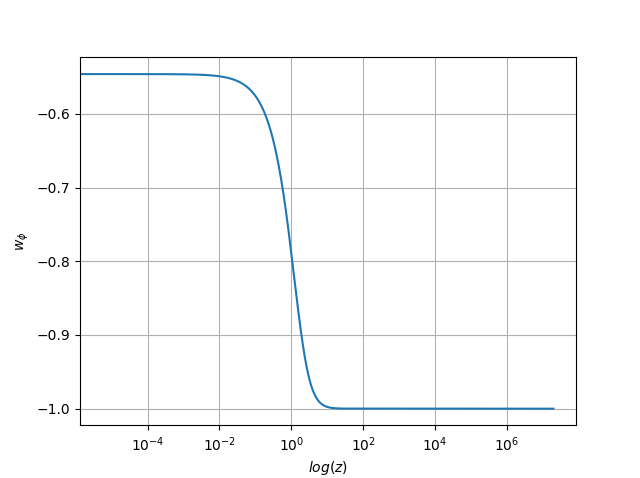
\includegraphics[width=12cm]{eos_exp.png}
\caption{Equation of state of the scalar field for exponential potential.}
\label{fig:eos_exp}
\end{figure}


\subsection{Hubble rate}
To evaluate the integral in equation (10*) we change the variable to N. We have that $N = \ln(a/a_0) = \ln(1/(1+z))$, so we have $z = e^{-N} - 1$ and $dz/dN = -e^{-N}$. The limits are easily calculated, inserting $z = z$ in $N = \ln(1/(1+z))$ yields just that, same procedure for $z=0$ yields 0. The integral then becomes

\begin{align}
\int_0^{\ln(\frac{1}{1+z})}\frac{3(1+w_{\phi}}{e^{-N}}(-e^{-N})dN = -\int_0^{\ln(\frac{1}{1+z})}3(1+w_{\phi}) dN.
\end{align}

Solving the Hubble rate numerically we divide by $H_0^2$ so that the equation is dimensionless. The equation then becomes

\begin{align}
\frac{H^2}{H_0^2} = \Omega_{r0}(1+z)^4 + \Omega_{m0}(1+z)^3 + \Omega_{\phi 0}\bigg(-\int_0^{\ln(\frac{1}{1+z})}3(1+w_{\phi})dN\bigg).
\end{align}

The plots are found in figure \ref{fig:h_rate_ipl} and \ref{fig:h_rate_exp}, the Hubble rate for the $\Lambda CDM$ model have also been added as figure \ref{fig:h_rate_lcdm}. We can see in all the plots that the time derivative of the scale factor becomes lower, and ultimately vanishes, as the redshift vanishes.


\begin{figure}[H]
\centering
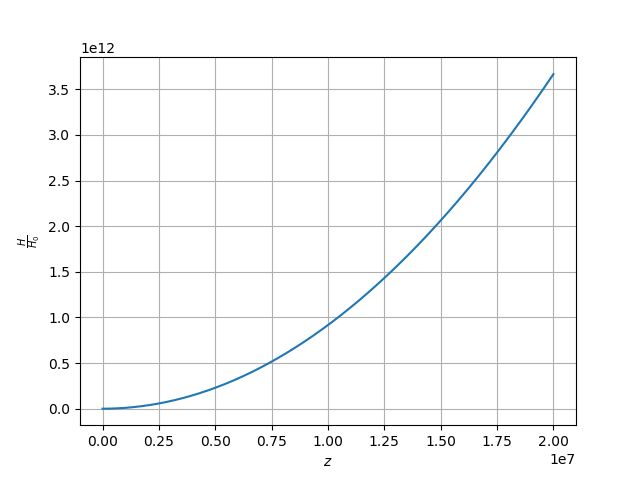
\includegraphics[width=12cm]{H_rate_ipl.png}
\caption{Hubble rate for the inverse power law potential.}
\label{fig:h_rate_ipl}
\end{figure}
\begin{figure}[H]
\centering
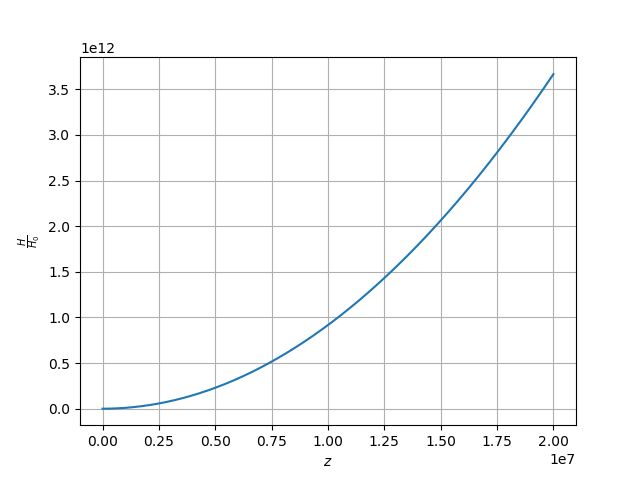
\includegraphics[width=12cm]{H_rate_exp.png}
\caption{Hubble rate for the exponential potential.}
\label{fig:h_rate_exp}
\end{figure}
\begin{figure}[H]
\centering
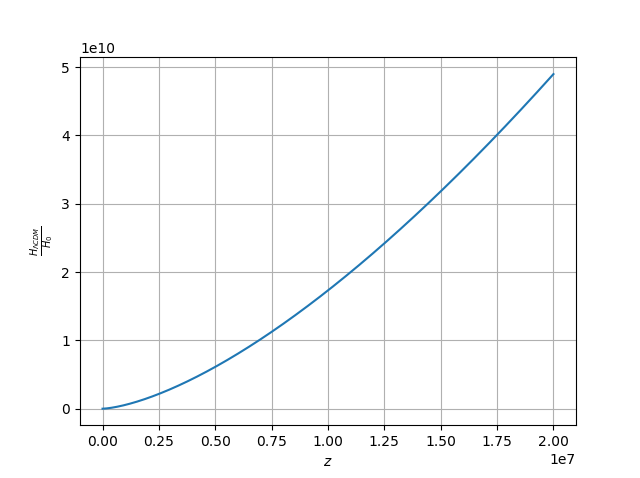
\includegraphics[width=12cm]{H_rate_LCDM.png}
\caption{Hubble rate for the $\Lambda CDM$ model.}
\label{fig:h_rate_lcdm}
\end{figure}

\subsubsection{Comments} The plots for the two potential models are identical, which tells me that it is independent of the potential, so I know something is wrong. I have tried numerical integration with Scipy's quad, trapezoidal and Simpson's method, but they all resulted in the same. I tried for loops where the calculation numerically goes as

\begin{align}
\frac{H^2}{H_0^2} = \Omega_{r0}(1+z_i)^4 + \Omega_{m0}(1+z_i)^3 + \Omega_{\phi 0}\bigg(-\int_0^{N_i}3(1+w_{\phi i})dN\bigg),
\end{align}

where $N_i = \ln(1/(1+z_i))$. I am not sure the error lies here, or in the integration of the $x_i$'s, but I doubt it is the latter. I have added failed (or working, to some degree) code at the bottom of the script. 


\subsection{$H_0t_0$}
We can find the age of the universe by

\begin{align}
t_0 = \int_0^{a_0} \frac{da}{a}H(a).
\end{align}

We wish to substitute so that the integral is taken over N. By the definition of N we get $a = e^Na_0$, and $da/dN = e^Na_0$. We finds the limits by the definition of N: $N(a_0) = \ln(a_0/a_0) = 0$ and $N(0) = \ln(0)$, for the latter we choose the lowest value of N. Multiplying by $H_0$ we get

\begin{align}
H_0t_0 = \int_{N_0}^0 \frac{e^Na_0}{e^Na_0 H/H_0}dN = \int_{N_0}^0 \frac{1}{H/H_0} dN.
\end{align}

For the inverse power law potential we find that the value is $H_0t_0 = 1.21$, for the exponential potential $H_0t_0 = 1.08$ and for the $\Lambda CDM$ model $H_0t_0 = 0.96$. We see again that the exponential potential provides the best model.

\subsubsection{Comments}
In this task I got different results based on whether I used Simpson's method or quad for numerical integration. The latter provided $H_0t_0 \approx 0.7$, but proved unsuccessful in the next task, yielding a luminosity distance of hundreds of thousands up to millions. There is a sketch of the code under the function "H0t0" as well as "H0t0\_quad" in the failed section of the script.

\subsection{Luminosity distance}
The luminosity distance is given by
\begin{align}
d_L = a_0(1+z)\frac{c}{H_0}\int_0^z \frac{dz'}{H/H_0}.
\end{align}

For the inverse power law potential $d_L = -4.83\frac{c}{H_0}$ and for the exponential potential $d_L = -4.74\frac{c}{H_0}$. If we ignore the large red blinking light, we could take the absolute value and simply conclude that yet again, the exponential potential is the victorious. For the $\Lambda CDM$ model $d_L = -0.79\frac{c}{H_0}$,

\section*{Final comments}
At this point I am unable to locate the exact source of the error, I have tried multiple methods of performing the definite integrals numerically, and varied these methods separately. I think it has something to do with the numerical integration using Simpson's method that is messing up the indexes. I tried to take this into consideration using SciPy quad to no avail. I tried rewriting code many times instead of editing once I got fresh ideas, but the results were too often similar to previous attempts, or way off. 



\begin{thebibliography}{9}

\bibitem{lamport94}
  Øystein Elgarøy,
  \textit{AST3220 - Cosmology I},
  \url{http://www.uio.no/studier/emner/matnat/astro/AST3220/v18/undervisningsmateriale/lectures.pdf} (downloaded 09.04.18)

\end{thebibliography}










\end{document}